\label{sec:det}
Conventional ET based methodologies are extensively used as tools to perform reliability and safety assessment of complex and critical engineering systems. 
One of the disadvantages of these methods is that timing/sequencing of events and system dynamics are not explicitly accounted for in the analysis.

%A PRA analysis needs an approximation to this distribution for selected consequence variables. 
%A way to achieve this goal is through a DET approach.
\begin{figure}[h] 
  \centering
     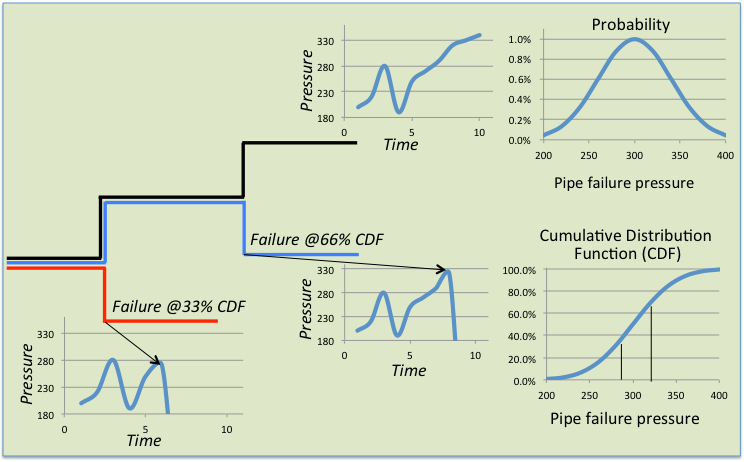
\includegraphics[width=0.73\textwidth]{figures/DET_schemeFlow.png}
  \caption{Dynamic Event Tree Conceptual Scheme.}
   \label{fig:DET_schemeFlow}
\end{figure}
In order to overcome these limitations a ``dynamic'' approach is needed. The DET technique brings several advantages~\cite{alfonsiPSA}~\cite{ADAPTHakobyan}, among which the fact that it simulates probabilistic system evolution in a way that is consistent with the severe accident model. In DET,  event sequences are run simultaneously starting from a single initiating event. The branchings occur at user specified times/conditions and/or when an action is required by the operator and/or the system, creating a deterministic sequence of events based on the time of their occurrence (see Fig.~\ref{fig:DET_schemeFlow}). 

This leads to a more realistic and mechanistically consistent analysis of the considered system. DPRA, including  DET methodologies,  are designed to take the timing of events explicitly into account which can become very important especially when uncertainties associated to complex phenomena are considered. \\
The main idea of this methodology is to let a system code (i.e., RELAP-7) determine the pathway of an accident scenario within a probabilistic ``environment''. 

Figure~\ref{fig:DET_schemeFlow} schematically shows the DET logic. As already mentioned, the accident sequence starts with an initiating event. Based on an user defined branching logic, driven by \textbf{P}robabilistic \textbf{D}istribution \textbf{F}unctions (PDFs), an event occurs at a certain time instant. The simulation spawns $n$ different branches. In each of them, the branching event determines a different consequence (carrying on associated probabilities). Each sequence continues until another event occurs and a new set of branching is spawned. The simulation ends when an exit condition or a maximum mission time is reached.
